\documentclass[a4paper,12pt]{article}
\usepackage{HomeWorkTemplate}

\usepackage[utf8]{inputenc}
\usepackage[]{babel}

\setlength{\parindent}{4em}
\setlength{\parskip}{0.5em}

\renewcommand{\baselinestretch}{1.5}

\usepackage{float} 
\usepackage{caption}
\usepackage{subcaption}
\usepackage{amsmath}
\usepackage[utf8]{inputenc}
\usepackage{lmodern, textcomp}
\usepackage{circuitikz}
\usepackage[shortlabels]{enumitem}
\usepackage{hyperref}
\usepackage{tikz}
\usepackage{amsmath}
\usepackage{amssymb}
\usepackage{tcolorbox}
\usepackage{graphicx}
\usepackage{xepersian}
\settextfont{XB Niloofar}
\usetikzlibrary{arrows,automata}
\usetikzlibrary{circuits.logic.US}
\usepackage{changepage}
\newcounter{problemcounter}
\newcounter{subproblemcounter}
\setcounter{problemcounter}{1}
\setcounter{subproblemcounter}{1}
\newcommand{\problem}[1]
{
	\subsection*{
		پرسش
		\arabic{problemcounter} 
		\stepcounter{problemcounter}
		\setcounter{subproblemcounter}{1}
		#1
	}
}
\newcommand{\subproblem}{
	\textbf{\harfi{subproblemcounter})}\stepcounter{subproblemcounter}
}


\begin{document}
\handout
{اصول پردازش تصویر}
{دکتر مصطفی کمالی تبریزی}
{نیم‌سال اول 1399\lr{-}1400}
{اطلاعیه}
{سیدعلیرضا خادم}
{97100398}
{تمرین سری دوم - سوال دوم}
\section*{موارد لازم.}
برای اجرا لازم است تا تصاویر
\lr{greek\_ship.jpg}
و
\lr{patch.png}
در مسیر
\lr{EX2\_Q2/images/}
قرار داشته باشد.
\section*{روند کلی حل.}
در ابتدا سعی شد حل این سوال با روش 
\lr{SSD}
انجام شود اما با توجه به اینکه نتیجه نتیجه خوبی با این روش به دست نمی‌آمد سراغ روش
\lr{normalized cross correlation}
 رفتیم. در این روش نتیجه بهتری نسبت به روش‌های
 \lr{cross correlation}
 ،
 \lr{zero mean cross correlation}
 و 
 \lr{SSD}
 حاصل می‌شد اما زمان اجرا در روش
 \lr{NCC}
 نسبت به روش‌های دیگر بیشتر بود، در نتیجه همان طور که در توضیح تابع هم
 \lr{normalized\_cross\_correlation}
 آمده است  به جای 
 \lr{$\overline{f_{m,n}}$}
  در رابطه‌یِ محاسبه 
  \lr{NCC}
  ،‌ میانگین کلِ عکس را قرار دادیم تا محاسبه عبارت در زمان خطی انجام شود و نتیجه هم خوب بود. نتیجه‌هایی که می‌شد گرفت تا حد خوبی بهتر شده بود اما به دلیل اینکه در 
  \lr{patch}
  علاوه بر ستون، قسمتی از آسمان و دریا هم وجود داشت نتیجه‌ای که در تصویر 
  \lr{000.jpg}
  در مسیر
  \lr{EX2\_Q2/images/}
  مشاهده می‌کنید به دست می‌آمد؛ در نتیجه تصمیم بر این شد تا با یک روشی 
  \lr{patch}
  را کوچکتر کنیم تا قسمت‌هایی اضافی حذف بشه. با انجام این کار با روش‌ای که در تابع 
   \lr{cut\_object\_of\_patch}
   توضیح داده شده به 
   \lr{001.jpg}
    در مسیر
   \lr{EX2\_Q2/images/}
   رسیدیم. در گام بعدی برای این که نتیجه بهتری به دست بیاید نتیجه 
   \lr{Template Matching}
   کانال‌های رنگی مختلف از 
   \lr{patch}
   و تصویر اصلی را مقایسه کردیم. تصویر
   \lr{003.jpg}
   ،
   \lr{004.jpg}
   و
   \lr{005.jpg}
    در مسیر
   \lr{EX2\_Q2/images/}
   به ترتیب مربوط به کانال‌های آبی، سبز و قرمز هستند. همانطور که مشاهده می‌کنید کانال آبی نتیجه بهتری میتواند بدهد، در نتیجه کانال آبی به عنوان مبنا در نظر گرفته شد. در نهایت هم یک
   \r{Gamma Transformation}
   روی نتیجه نهایی اعمال شد تا اون قسمت‌هایی که کاندید‌های اصلی بودند روشن تر شوند و در عوض اون قسمت‌هایی که کاندیدا نبودن تیره بشوند و تصویر 
   \lr{gamma\_trans\_applyed.jpg}
   در مسیر
   \lr{EX2\_Q2/images/}
   به دست آمد.
  
  در این کد تعداد 
  \lr{object}
  هایی که در تصویر میخواهیم دیتکت بشوند را در متغیر 
  \lr{number\_of\_object}
  در فایل 
  \lr{utilities.py}
  باید مشخص کنیم. برای مثال در این سوال تعداد این 
  \lr{object}
  ها 9 عدد است که شامل 4 ستون در آب و 5 ستون روی کشتی می‌شود.
  
  در آخر هم باید به این نکته اشاره کنم که برای حل این سوال به این نکته توجه شده بود که ممکن است سایز 
  \lr{object}
  هایی که در تصویر هستند و قرار است دیتکت شوند با سایز 
   \lr{template}
   متفاوت باشد که در این صورت یک راهکاری که وجود دارد سرچ کردن 
   \lr{template}
   با سایزهای متفاوت است. در این سوال در ابتدا پیاده سازی این موضوع انجام شده بود اما با توجه به اینکه در این سوال استثنائا بدون این کار هم نتیجه مطلوبی حاصل شد. آن بخش از پیاده‌سازی حذف گردید.
\section*{توضیح کد.}
برنامه در مجموع حاوی 2 فایل با فرمت
\lr{.py}
می‌باشد که توضیحات هر فایل در پایین آمده است.
\subsection*{$\circ$ utilities.py}
\subsubsection*{canny(src\_image)}
این تابع تصویر
\lr{src\_image}
را به عنوان ورودی می‌گیرد و متد تشخیص مرزِ
\lr{canny}
را با 
\lr{high\_thresh}
و
\lr{low\_thresh}
ای که در تابع محاسبه شده است روی آن اعمال می‌کند و تصویری که حاصل می‌شود را به عنوان خروجی بر‌می‌گرداند.
\subsubsection*{\lr{cut\_object\_of\_patch(gray\_template\_patch, template\_patch)}}
هدف از پیاده سازی این تابع این بوده است که 
\lr{template}
ای که در سوال داده شده بود  علاوه بر ستون‌ (‌که 
\lr{object}
اصلی ای بود که باید تشخیص داده می‌شد) قسمتی از آسمان و دریا هم در 
 \lr{template}
 و جود داشت و با این باعث می‌شد که نتیجه خوبی به حاصل نشه. این تابع 
 \lr{gray\_template\_patch}
 که نسخه سیاه و سفید 
 \lr{template}
 داده شده در سوال است و 
 \lr{template\_patch}
 که همان 
 \lr{template}
 داده شده در سوال است را به عنوان ورودی می‌گیرد و با استفاده از تابع 
 \lr{canny()}
 مرز های 
  \lr{gray\_template\_patch}
 را همان طور که در تصویر 
  \lr{template\_edge\_detected.jpg}
  در مسیر 
  \lr{EX2\_Q2/images/}
  قابل مشاهده است به دست می‌آورد. سپس کوچکترین مستططیلی که شامل مرزهای تشخیص داده شده است را محاسبه می‌کند و آن قسمت از تصویرِ
  \lr{template\_patch}
 را (منظور از قسمت همان مستطیل‌ای است که محاسبه شده) همان طور که در تصویر 
 \lr{new\_patch.png}
 در مسیر
 \lr{EX2\_Q2/images/}
 قابل مشاهده است به عنوان خروجی برمی‌گرداند.
 \subsubsection*{\lr{normalized\_cross\_correlation(src\_image, input\_template)}}
 در این تابع پیاده‌سازی روش 
\lr{normalized cross correlation}
برای 
\lr{Template Matching}
انجام شده، با این تفاوت که در عبارتی که برای 
\lr{normalized cross correlation}
 در اسلاید‌های درس آمده و در پایین هم تصویر عبارت قرار داده شده است، به جای 
 \lr{$\overline{f_{m,n}}$}
 ،‌ میانگین کلِ عکس را قرار دادیم تا محاسبه عبارت در زمان خطی انجام شود (‌باید در نظر داشت که این کار مشروط  به اینکه در ریزالت نهایی تاثیر منفی نداشته باشه انجام شده). درنهایت هم 
 \lr{result}
 اسکیل شده به 0 تا 255 و به عنوان خروجی باز گردانده شده است.
  \begin{figure}[H]
 	\centering
 	\begin{subfigure}{0.9\textwidth}
 		\centering
 		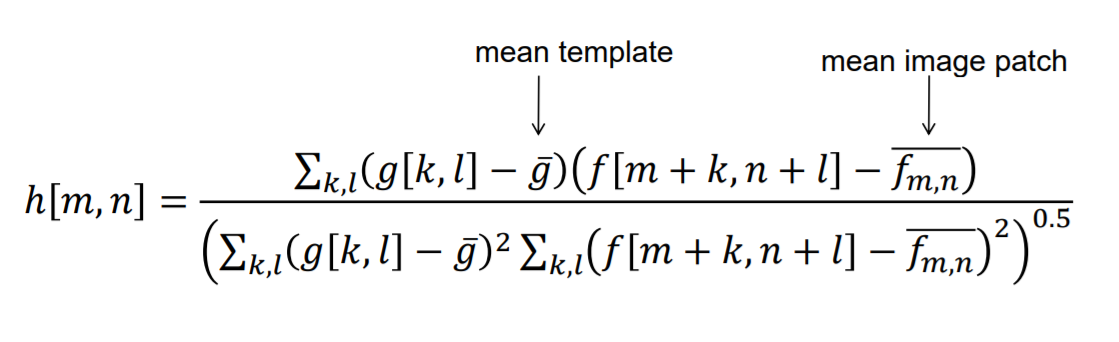
\includegraphics[width=\textwidth]{eq.png}
 	\end{subfigure}
 \end{figure}
 \subsubsection*{\lr{draw\_rectangle\_aroung\_detected\_template(src\_image, result, w, h , k)}}
 این تابع 
 \lr{src\_image}
 را به عنوان عکسی که قرار است در آن دور 
 \lr{object}
 های تشخیص داده شده مستطیل رسم شود ، 
 \lr{result}
 را به عنوان نتیجه 
 \lr{normalized cross correlation}
 ،
 \lr{w}
 و
 \lr{h}
 را به عنوان ابعاد 
  \lr{template}
   و 
   \lr{k }
   را به عنوان تعداد اشیایی که در عکس وجود دارد ورودی می‌گیرد و 
   \lr{for}
   ای می‌زند که تعداد اجرای آن 
   \lr{k}
   بار است و در هر بار اجرا نگاه می‌کند ماکزیممِ
   \lr{result}
   کجا قرار دارد، به مرکز آن نقطه یک مستطیل رسم می‌کند و یک ناحیه‌ای اطراف آن را مقادیرشان را مقدار کمی قرار می‌هد تا در اجراهای بعدی حلقه دیگر در آن قسمت‌ها 
   \lr{object}
   ای دیتکت نشود.
   \subsubsection*{\lr{apply\_gamma\_transformation(src\_image, gamma)}}
   این تابع یک تصویر را به عنوان ورودی می‌گیرد و یک 
   \lr{Gamma Transformation}
   روی آن اعمال می‌کند و نتیجه اعمال را به عنوان خروجی بر‌می‌گرداند.
\subsection*{$\circ$ q2.py}
در این فایل ابتدا تصاویر 
\lr{greek\_ship.jpg}
و 
\lr{patch.jpg}
را از مسیر
\lr{EX2\_Q2/images/}
لود شده است. بعد برای جلوگیری از 
\lr{overflow}
شدن مقادیر قرمت 
\lr{src\_image}
و 
\lr{template}
به 
\lr{np.float\_}
تغییر داده شده است. در ادامه با توجه به توضیاحتی که در 
\textbf{روند کلی حل.}
و
\textbf{توضیح کد.}
داده شد 
\lr{result}
محاسبه می‌شود و تحت عنوان 
\lr{res03.jpg}
در مسیر
\lr{EX2\_Q2/results/}
ذخیره می‌شود.


\end{document}
